\tikzset{
    ultra thin/.style= {line width=0.1pt},
    very thin/.style=  {line width=0.2pt},
    thin/.style=       {line width=0.4pt},% thin is the default
    semithick/.style=  {line width=0.6pt},
    thick/.style=      {line width=0.8pt},
    very thick/.style= {line width=1.2pt},
    ultra thick/.style={line width=1.6pt}
}
\definecolor{mintbg}{rgb}{.63,.79,.95}

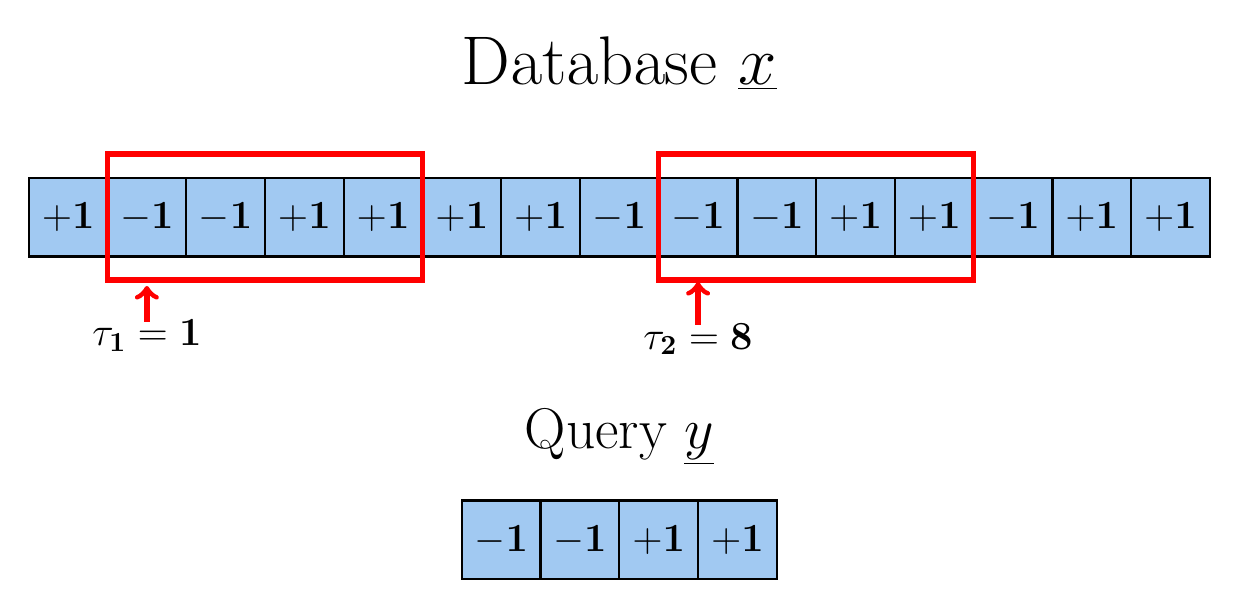
\begin{tikzpicture}

\draw[thick, fill = mintbg]  (-15.5,12.05) rectangle (-0.5,11.05);
\draw[thick]  (-14.5,12.05) rectangle (-14.5,11.05);
\draw[thick]  (-13.5,12.05) rectangle (-13.5,11.05);
\draw[thick]  (-12.5,12.05) rectangle (-12.5,11.05);
\draw[thick]  (-11.5,12.05) rectangle (-11.5,11.05);
\draw[thick]  (-10.5,12.05) rectangle (-10.5,11.05);
\draw[thick]  (-9.5,12.05) rectangle (-9.5,11.05);
\draw[thick] (-8.5,12.05) rectangle (-8.5,11.05);
\draw[thick]  (-7.5,12.05) rectangle (-7.5,11.05);
\draw[thick]  (-6.5,12.05) rectangle (-6.5,11.05);
\draw[thick]  (-5.5,12.05) rectangle (-5.5,11.05);
\draw[thick]  (-4.5,12.05) rectangle (-4.5,11.05);
\draw[thick]  (-3.5,12.05) rectangle (-3.5,11.05);
\draw[thick]  (-2.5,12.05) rectangle (-2.5,11.05);
\draw[thick]  (-1.5,12.05) rectangle (-1.5,11.05);
\node at (-15,11.55) {\Large $\bf  +1$};
\node at (-14,11.55) {\Large$\bf -1$};
\node at (-13,11.55) {\Large$\bf -1$};
\node at (-12,11.55) {\Large$\bf +1$};
\node at (-11,11.55) {\Large$\bf +1$};
\node at (-10,11.55) {\Large$\bf +1$};
\node at (-9,11.55) {\Large$\bf +1$};
\node at (-8,11.55) {\Large$\bf -1$};
\node at (-7,11.55) {\Large$\bf -1$};
\node at (-6,11.55) {\Large$\bf -1$};
\node at (-5,11.55) {\Large$\bf +1$};
\node at (-4,11.55) {\Large$\bf +1$};
\node at (-3,11.55) {\Large$\bf -1$};
\node at (-2,11.55) {\Large$\bf +1$};
\node at (-1,11.55) {\Large$\bf +1$};

\node at (-8,13.5) {\Huge Database  $\underline{x}$};



\node at (-8,8.75) {\huge Query  $\underline{y}$};

\draw[thick, fill = mintbg] (-10,7.95) rectangle (-6,6.95);
\draw[thick]  (-9,7.95) rectangle (-9,6.95);
\draw[thick]  (-8,7.95) rectangle (-8,6.95);
\draw[thick]  (-7,7.95) rectangle (-7,6.95);

\node at (-9.5,7.45) {\Large$\bf -1$};
\node at (-8.5,7.45) {\Large$\bf -1$};
\node at (-7.5,7.45) {\Large$\bf +1$};
\node at (-6.5,7.45) {\Large$\bf +1$};

 \node (v3) at (-7,10.85) {};
 \node (v4) at (-7,10.05) {};
\draw[<-, line width = 2pt, color = red]  (v3) edge (v4);
\node at (-7,10) {\Large$\bf \tau_2 = 8$};

\draw[line width = 2pt, color = red]  (-14.5,12.35) rectangle (-10.5,10.75);
\draw[line width = 2pt, color = red]  (-7.5,12.35) rectangle (-3.5,10.75);
\node (v1) at (-14,10.8) {};
\node (v2) at (-14,10.1) {};
\draw[<-, line width = 2pt, color = red]  (v1) edge (v2);
\node at (-14,10.05) {\Large$\bf  \tau_1 = 1$};



\end{tikzpicture}